\documentclass{article}
\usepackage[utf8]{inputenc}
\usepackage{enumitem}
\usepackage{amsmath,amsthm,amssymb}
\usepackage[english]{babel}
\usepackage[a4paper, portrait, margin=1.2in]{geometry}
% \usepackage{ntheorem}
% \usepackage{theoremref}
\usepackage{xifthen}
\usepackage{relsize}
\usepackage[svgnames]{xcolor} % You can find CSS colours here https://www.w3schools.com/cssref/css_colors.asp

\usepackage{tkz-euclide}
\usepackage{tikz}
% \usepackage{showframe} % Useful for debugging

\usepackage{titlesec}
% \usepackage{caption}
\definecolor{MainColor}{hsb}{0, 0.8, 0.65}
\definecolor{SubColor}{hsb}{0.01, 0.90, 0.45}
\definecolor{SubSubColor}{hsb}{0.01, 0.90, 0.2}
% \usepackage[labelfont={color=SubColor,bf}]{caption}
\usepackage[labelfont={color=SubColor,bf}]{caption}

\title{Factorizing Polynomials Part 1}
\author{Rasmus Söderhielm}
\date{January 2022}

% \parindent 20pt
% \parskip 1em


% switch implementation from https://tex.stackexchange.com/questions/64131/implementing-switch-cases
\newcommand{\ifequals}[3]{\ifthenelse{\equal{#1}{#2}}{#3}{}}
\newcommand{\case}[2]{#1 #2} % Dummy, so \renewcommand has something to overwrite...
\newenvironment{switch}[1]{\renewcommand{\case}{\ifequals{#1}}}{}

\newcommand{\hint}{\\\textcolor{SubColor}{{H}{\relsize{-1}INT:}}\ }



\renewcommand*{\thesubsection}{\textcolor{MainColor}{\Alph{subsection}}}
\renewcommand*{\thesubsubsection}{\textcolor{MainColor}{\arabic{subsubsection}}}
% \renewcommand*{\subsection}[1]{\thesubsection #1}

\newcommand{\solution}{\subsubsection*{\textcolor{MainColor}{Solution}}}

\newcounter{theoremcounter}

\newtheoremstyle{maintheorem}% name of the style to be used
	{\topsep}% measure of space to leave above the theorem. E.g.: 3pt
	{\topsep}% measure of space to leave below the theorem. E.g.: 3pt
	{\itshape}% name of font to use in the body of the theorem
	{0pt}% measure of space to indent
	{\color{SubColor}\bfseries}% name of head font
	{.}% punctuation between head and body
	{ }% space after theorem head; " " = normal interword space
	{\thmname{#1}\thmnumber{ #2}\textnormal{\thmnote{ (#3)}}}

\theoremstyle{maintheorem}
\newtheorem{theorem}[theoremcounter]{\textcolor{SubColor}{Theorem}}
\newtheorem{corollary}{\textcolor{SubColor}{Corollary}}


\newcommand{\thmref}[1]{\textcolor{SubSubColor}{\textbf{Theorem \ref{#1}}}}
\newcommand{\corref}[1]{\textcolor{SubSubColor}{\textbf{Corollary \ref{#1}}}}
\renewcommand{\eqref}[1]{\textcolor{SubSubColor}{\textbf{Equation \ref{#1}}}}

% \theoremstyle{mainsolution}
% \newtheorem*{solution}{Solution}



\newcommand{\size}[2]{
	\begin{switch}{#1}
		\case{1}{#2}
		\case{2}{\bigl#2}
		\case{3}{\Bigl#2}
		\case{4}{\biggl#2}
		\case{5}{\Biggl#2}
	\end{switch}
}

\setlength{\parskip}{0.8em}

\begin{document}

\linespread{1.5}\selectfont

\maketitle

\section*{\color{MainColor}Problems} \label{Problems}
\subsection{
    A basic geometric proof
}
Let $\alpha$, $\beta$, $\gamma$, $\delta$ and $\epsilon$ be the angles of a pentagon
whose vertices are arranged into any arbitrary star like shape.
Let $\theta$ be the sum of the these angles.
Is $\theta$ constant, and if it's not, then why?

\begin{figure}[h]\label{star}
    \centering
    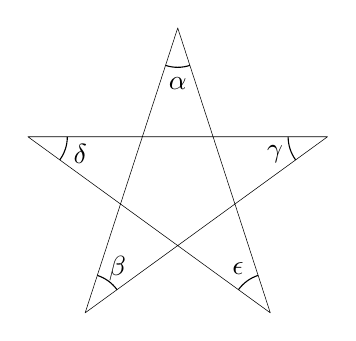
\begin{tikzpicture}[x=1cm,y=1cm]

        \foreach \an\letter in {90/A,162/D,234/B,306/E,378/C}
            { \tkzDefPoint(\an:2){\letter}}
        \tkzDrawPolygon(A,B,C,D,E)
        % \tkzDrawPoints(A,B,C,D,E)

        \tkzMarkAngle[size=0.5,mark=none](B,A,E)
        \tkzLabelAngle[pos=0.7](B,A,E){$\alpha$}
        \tkzMarkAngle[size=0.5,mark=none](C,B,A)
        \tkzLabelAngle[pos=0.7](C,B,A){$\beta$}
        \tkzMarkAngle[size=0.5,mark=none](D,C,B)
        \tkzLabelAngle[pos=0.7](D,C,B){$\gamma$}
        \tkzMarkAngle[size=0.5,mark=none](E,D,C)
        \tkzLabelAngle[pos=0.7](E,D,C){$\delta$}
        \tkzMarkAngle[size=0.5,mark=none](A,E,D)
        \tkzLabelAngle[pos=0.7](A,E,D){$\epsilon$}
    \end{tikzpicture}

    \caption{The aforementioned pentagon whose sum of angles is sought after.}
\end{figure}

\solution

Let's begin by imageing the angles created by the points of intersection of our star's sides
and the pentagon formed by these points of intersection.
We will call these angles $a_1$ and $a_2$ for $a$ through $e$,
with $a_1$ defined as the exterior angle and $a_2$ defined as the interior angle of the pentagon.

\end{document}